\chapter{Weryfikacja systemu, wyzwania i wnioski}
\label{cha:verification}

Ostatnia część pracy łączy weryfikację poprawności i bezpieczeństwa zaimplementowanego systemu, omówienie napotkanych problemów technicznych wraz z ich rozwiązaniami oraz podsumowanie uzyskanych rezultatów. Takie ujęcie pozwala oddzielić testy funkcjonalne od analizy wydajnościowej --- która bezpośrednio wynika z wyzwań związanych z integracją modeli \gls{LLM} --- i zakończyć pracę spójnymi wnioskami.

\section{Testy poprawności i bezpieczeństwa}
Proces weryfikacji poprawności działania systemu został podzielony na testy automatyczne warstwy backendowej, testy manualne interfejsu użytkownika, testy \gls{E2E} oraz audyt bezpieczeństwa. Takie podejście pozwoliło na wykrycie błędów zarówno na poziomie logicznym, jak i funkcjonalnym.

\subsection{Testy jednostkowe i integracyjne backendu}
Warstwa serwerowa aplikacji, zaimplementowana w języku Python, została pokryta testami automatycznymi przy użyciu frameworka \texttt{pytest}. Głównym celem tych testów była weryfikacja poprawności działania poszczególnych endpointów \gls{API} oraz logiki biznesowej generatora danych.

Testy, zlokalizowane w katalogu \texttt{backend/tests}, obejmują następujące scenariusze:
\begin{itemize}
    \item Weryfikacja autentykacji: Sprawdzenie poprawności generowania i walidacji tokenów \gls{JWT}. Testy upewniają się, że dostęp do chronionych zasobów bez ważnego tokenu jest blokowany (kod błędu 401 Unauthorized).
    \item \gls{CRUD} projektów: Testowanie operacji tworzenia, odczytu i usuwania projektów. Weryfikowana jest poprawność zapisu struktury \gls{JSON} do bazy danych PostgreSQL.
    \item Walidacja schematów Pydantic: Sprawdzenie, czy system poprawnie odrzuca błędne żądania (np. brak wymaganych pól, niepoprawne typy danych).
    \item Symulacja generowania danych: Uruchamianie silnika generującego dla prostych konfiguracji w celu potwierdzenia, że zwracane dane są zgodne z zadeklarowanym typem.
\end{itemize}

Przykładowy test weryfikujący działanie endpointu \texttt{/generate} wygląda następująco:
\begin{verbatim}
def test_generate_endpoint(client, auth_headers):
    payload = {
        "config": {"job_name": "Test Job", "rows": 10},
        "tables": [...]
    }
    response = client.post("/generate", json=payload, headers=auth_headers)
    assert response.status_code == 200
    data = response.json()
    assert "status" in data
    assert data["status"] == "success"
\end{verbatim}

\subsection{Testy manualne interfejsu użytkownika}
Ze względu na dynamiczny charakter interfejsu, duży nacisk położono na testy manualne. Scenariusze testowe obejmowały pełne ścieżki użytkownika (ang. \emph{User Journeys}).

\subsubsection*{Scenariusz 1: Utworzenie schematu sklepu internetowego}
Celem tego testu było sprawdzenie integralności relacyjnej generowanych danych.
\begin{enumerate}
    \item Utworzenie tabeli \texttt{users} z polami \texttt{id}, \texttt{name}, \texttt{email}.
    \item Utworzenie tabeli \texttt{orders} z polem \texttt{user\_id} jako klucz obcy do tabeli \texttt{users}.
    \item Uruchomienie generowania dla 100 użytkowników i 500 zamówień.
    \item Weryfikacja: Sprawdzenie, czy każde zamówienie przypisane jest do istniejącego użytkownika. Test zakończył się sukcesem --- silnik poprawnie rozwiązał zależności w 100\% przypadków.
\end{enumerate}

\subsubsection*{Scenariusz 2: Integracja z LLM}
Testowano zachowanie systemu przy generowaniu pól typu \texttt{llm} oraz poprawność obsługi asynchronicznego postępu zadania.
\begin{enumerate}
    \item Zdefiniowanie pola typu \texttt{llm} z promptem generującym opis produktu.
    \item Ustawienie liczby wierszy na 50.
    \item Obserwacja: Interfejs pozostawał responsywny podczas oczekiwania na odpowiedź z \gls{API} OpenAI, a pasek postępu aktualizował się w czasie rzeczywistym. Po zakończeniu zadania wygenerowano kompletny zestaw rekordów zgodny ze schematem. Szczegóły pomiarów wydajnościowych oraz optymalizacji opisano w Sekcji \ref{sec:llm_optimization}.
\end{enumerate}

\subsection{Testy End-to-End (\texorpdfstring{\gls{E2E}}{E2E})}
W celu weryfikacji integralności całego systemu wprowadzono testy typu \gls{E2E}, symulujące rzeczywiste scenariusze użytkowania --- od interfejsu w przeglądarce, przez warstwę \gls{API}, aż po logikę biznesową i bazy danych.

Do realizacji testów \gls{E2E} wybrano framework Playwright. Jest on nowoczesnym narzędziem umożliwiającym automatyzację testów w wielu przeglądarkach (Chromium, Firefox, WebKit) oraz zapewniającym wysoką niezawodność dzięki mechanizmom automatycznego oczekiwania na elementy interfejsu.

Zaimplementowany scenariusz testowy pokrywa kluczową ścieżkę krytyczną \cite{happy_path} użytkownika:
\begin{enumerate}
    \item Autoryzacja: Scenariusz rozpoczyna się od wejścia na stronę logowania. Automat testowy wprowadza dane uwierzytelniające administratora i weryfikuje poprawne przekierowanie do głównego widoku aplikacji.
    \item Definicja schematu: Wirtualny użytkownik dodaje nową tabelę o nazwie ,,users'' oraz konfiguruje jej strukturę, dodając kolumnę ,,name''. Test weryfikuje poprawność interakcji z formularzami oraz dynamiczne aktualizacje interfejsu.
    \item Generowanie danych: Następuje uruchomienie procesu generowania danych poprzez kliknięcie przycisku ,,Run Generation''. Test monitoruje asynchroniczny proces, oczekując na komunikaty o postępie przekazywane przez WebSocket.
    \item Weryfikacja wyników: Ostatnim krokiem jest potwierdzenie zakończenia zadania sukcesem (pojawienie się komunikatu ,,Data generated!'') oraz sprawdzenie dostępności przycisku pobierania wyników.
\end{enumerate}

Dzięki zastosowaniu symulowania odpowiedzi backendu w wybranych testach możliwe jest izolowane testowanie warstwy frontendowej, co przyspiesza proces deweloperski i uniezależnia testy interfejsu od dostępności zewnętrznych usług czy modeli \gls{LLM}.

\subsection{Testy bezpieczeństwa}
\input{sections/security_testing_body.tex}


\section{Wyzwania implementacyjne}
Stworzenie aplikacji łączącej konwencjonalne generowanie danych z wykorzystaniem modeli sztucznej inteligencji wiązało się z szeregiem problemów technicznych. Poniżej opisano najistotniejsze z nich oraz przyjęte rozwiązania --- z wyjątkiem kwestii wydajności generowania przez \gls{LLM}, które ze względu na swój zasięg omówiono osobno w kolejnej sekcji.

\subsection{Informowanie użytkownika o postępie}
Jednym z istotnych problemów na początku prac było płynne wyświetlanie paska postępu generowania na stronie internetowej, podczas gdy cały proces odbywał się w tle na serwerze.

Standardowe zapytania \gls{HTTP} nie sprawdzają się najlepiej w tym zastosowaniu, ponieważ przeglądarka musiałaby nieustannie pytać serwer o aktualny status. Przy większej liczbie użytkowników spowodowałoby to znaczne przeciążenie sieci. Zdecydowano się na wykorzystanie protokołu WebSocket. W backendzie utworzono specjalny endpoint \texttt{/ws/jobs/\{job\_id\}}, do którego podłącza się aplikacja. Program działający w tle regularnie zapisuje swój postęp do pamięci współdzielonej, a połączenie WebSocket odczytuje te dane co pół sekundy i przesyła na bieżąco do przeglądarki. Dzięki temu interfejs działa responsywnie i płynnie aktualizuje pasek postępu.

\subsection{Wymuszanie unikalności danych z modelu LLM}
Modele językowe charakteryzują się niedeterministycznym działaniem, co stanowiło wyzwanie w przypadku generowania kolumn, dla których zaznaczono wymóg unikalności (np. dla numerów seryjnych generowanych przez AI).

Podczas testów zauważono, że przy ustawieniu wysokiej ,,temperatury'' (parametr \texttt{temperature}) model często tracił kontekst i nie trzymał się narzuconego formatu. Z kolei przy niskiej temperaturze wykazywał tendencję do generowania tych samych słów i schematów. Aby zapobiec powstawaniu duplikatów, zaimplementowano własny mechanizm weryfikacji:
\begin{enumerate}
    \item Aplikacja zapisuje w pamięci listę wygenerowanych wartości dla danej unikalnej kolumny.
    \item Przy każdej nowej odpowiedzi od sztucznej inteligencji następuje sprawdzenie, czy dana wartość nie została już wykorzystana.
    \item W przypadku wykrycia duplikatu system ponawia zapytanie (maksymalnie do 10 razy). Do promptu doklejana jest dodatkowa instrukcja: \texttt{CONSTRAINT: Value MUST be unique. DO NOT use: [lista wykorzystanych wartości]}.
    \item Aby pomóc modelowi w znalezieniu nowej odpowiedzi, przy kolejnych próbach aplikacja delikatnie zwiększa parametr \texttt{temperature} (+0.1), co zachęca algorytm do większej różnorodności w doborach słów.
\end{enumerate}

\subsection{Zależności cykliczne}
Aplikacja sortuje tabele przed generowaniem, aby zapewnić odpowiednią kolejność ich tworzenia (np. najpierw użytkownicy, potem ich opinie). Problem pojawiał się, gdy Tabela A wymagała klucza z Tabeli B, a Tabela B jednocześnie wymagała klucza z Tabeli A.

Tworzył się wówczas tzw. cykl zależności, który zapętlał program. Na obecnym etapie przyjęto założenie, że użytkownik musi świadomie projektować strukturę bazy i unikać takich sytuacji w interfejsie. W przyszłości planowane jest dodanie dodatkowej walidacji, która blokowałaby zapis schematu w przypadku wykrycia ,,błędnego koła''.

\subsection{Odporność na błędy łączności z API}
Komunikacja z zewnętrznymi interfejsami, takimi jak API usługi OpenAI, niesie ze sobą ryzyko sporadycznej utraty połączenia sieciowego lub przeciążeń po stronie dostawcy chmury. W kodzie serwera uodporniono wywołania API za pomocą precyzyjnych bloków wychwytywania wyjątków \texttt{try-except}. W przypadku wystąpienia \textit{timeoutu} (braku odpowiedzi sieciowej dla konkretnego zapytania) system nie odrzuca całego procesu po wielu godzinach pracy. Kod zachowuje odpowiedni tekst błędu (np. \texttt{Connection error}), wpisując go bezpiecznie w odpowiednią komórkę bazy danych tabeli. Pozwala to na płynne kontynuowanie generowania kolejnego wiersza, uniemożliwiając restart skryptu i pozostawiając operatorowi wgląd w omyłkowy element poprzez odnalezienie komunikatu błędu w docelowym pliku Excel bądź CSV.


\section{Wydajność i optymalizacja generowania}
\label{sec:llm_optimization}
Największym wyzwaniem dla wydajności systemu okazało się generowanie opisów przez modele \gls{LLM}. Początkowa wersja kodu zakładała przetwarzanie wierszy pojedynczo: program tworzył wiersz, wysyłał zapytanie do serwera Ollama, czekał na odpowiedź i dopiero wtedy przechodził do kolejnego rekordu.

Pomiary wykazały, że wygenerowanie 100 recenzji produktów przez model Llama 3 zajmowało blisko 130 sekund. Prawie 95\% tego czasu stanowiło oczekiwanie na odpowiedź sztucznej inteligencji, podczas gdy zwykłe dane tekstowe (np. nazwiska z biblioteki Faker) generowały się w ułamki sekund. Czas oczekiwania na jeden rekord wynosił około 1,3 sekundy, a procesor oraz karta graficzna przez większość tego czasu nie były w pełni obciążone.

\subsection*{Algorytm dwufazowy i przetwarzanie wsadowe}
W celu lepszego wykorzystania zasobów obliczeniowych wprowadzono algorytm dwufazowy:
\begin{enumerate}
    \item W pierwszej kolejności aplikacja generuje wszystkie standardowe wiersze dla tabeli, całkowicie pomijając kolumny LLM. Działa to natychmiastowo i tworzy gotowe obiekty, które mogą posłużyć jako kontekst dla zapytań AI.
    \item Zebrane konteksty są następnie przekazywane w paczkach do oddzielnej funkcji, która zajmuje się wyłącznie komunikacją z modelem.
\end{enumerate}

Kluczem do przyspieszenia procesu okazało się grupowanie zapytań w mniejsze pakiety. Zamiast wysyłać pojedynczy wiersz, program opiera się na parametrze \texttt{SUB\_BATCH\_SIZE} (domyślnie 15) i wysyła do modelu kilkanaście kontekstów w jednym dużym prompcie. W odpowiedzi model zwraca tekstową strukturę \gls{JSON} zawierającą od razu cały pakiet wyników, co skraca narzut czasu potrzebny na wielokrotne inicjalizowanie zapytań przez silnik AI.

Dodatkowo zastosowano mechanizm \texttt{asyncio.Semaphore}, który zezwala serwerowi Ollama na przetwarzanie kilku takich paczek jednocześnie (domyślnie 8 zapytań w tle). Jeśli wystąpi błąd formatowania dla danej paczki (np. model pominie znak w odpowiedzi \gls{JSON}), uszkodzony fragment jest wyłapywany i przerabiany bezpiecznym, pojedynczym zapytaniem, aby nie psuć całego postępu generowania.

\subsection*{Dobór parametrów optymalizacji}
W celu dobrania optymalnych parametrów przeprowadzono pięć pomiarów na stałej próbce 100 wierszy z polami generowanymi przez \gls{LLM}. Każda próba dotyczyła innego sposobu wysyłania zapytań do modelu. Pomiary wykonano na laptopie z kartą NVIDIA RTX 5060, z modelem Llama 3 w Ollama --- ten sam sprzęt i ta sama próbka we wszystkich wierszach tabeli.

\begin{table}[H]
    \centering
    \begin{tabular}{|c|c|p{7cm}|}
        \hline
        \textbf{Próba optymalizacji} & \textbf{Czas [s]} & \textbf{Sposób generowania}                              \\
        \hline
        1                            & 129,52            & Jeden wiersz na raz --- wersja początkowa                \\
        \hline
        2                            & 218,88            & Wiele równoległych zapytań, ale nadal po jednym wierszu  \\
        \hline
        3                            & 63,43             & Kilka wierszy łączonych w jedno zapytanie (pakietowanie) \\
        \hline
        4                            & 124,41            & Pakietowanie z niekorzystnymi rozmiarami paczek          \\
        \hline
        5                            & 52,24             & Pakietowanie po 15 wierszy, maksymalnie 8 zapytań naraz  \\
        \hline
    \end{tabular}
    \caption{Porównanie wariantów generowania 100 wierszy AI (Ollama, RTX 5060)}
    \label{tab:llm_optimization_100}
\end{table}

Tabela \ref{tab:llm_optimization_100} pokazuje, że sama równoległość (próba 2) bez grupowania wierszy pogarsza wynik --- serwer Ollama zostaje przeciążony i czas rośnie do 219 s. Dopiero połączenie wielu wierszy w jednym prompcie (próba 3) skraca czas do około 63 s. Próba 4 potwierdza, że rozmiar paczki ma znaczenie: przy złych ustawieniach czas wraca do poziomu wersji sekwencyjnej. Wariant docelowy (próba 5) łączy pakietowanie z umiarkowaną równoległością i daje około 52 s --- blisko 2,5-krotnie szybciej niż wersja początkowa.

\subsection*{Wpływ rozmiaru paczki na czas generowania}
Aby precyzyjnie ocenić, jak liczba wierszy łączonych w jednym zapytaniu wpływa na wydajność, przeprowadzono dodatkową serię pomiarów. Wygenerowano 100 rekordów z polem tekstowym obsługiwanym przez \gls{LLM}, zmieniając wyłącznie parametr \texttt{SUB\_BATCH\_SIZE} (1, 2, 5, 10, 20 i 100). We wszystkich próbach utrzymano \texttt{MAX\_CONCURRENT=1}, tak aby wynik zależał głównie od wielkości paczki, a nie od równoległości zapytań. Testy wykonano z wykorzystaniem chmurowego API OpenAI (zamiast lokalnej instancji Ollama), co pozwoliło sprawdzić zachowanie modelu w warunkach zbliżonych do typowego wdrożenia produkcyjnego.

\begin{table}[H]
    \centering
    \begin{tabular}{|c|c|c|}
        \hline
        \textbf{Rozmiar paczki} & \textbf{Czas [s]} & \textbf{Uwagi}                                                 \\
        \hline
        1                       & 90                & generowanie pojedyncze --- punkt odniesienia                   \\
        \hline
        2                       & 60                & widoczne przyspieszenie dzięki mniejszej liczbie zapytań       \\
        \hline
        5                       & 43                & dalszy spadek czasu                                            \\
        \hline
        10                      & 30                & najkrótszy czas --- optymalny zakres dla testowanego modelu    \\
        \hline
        20                      & 76                & model zwracał niepoprawną liczbę wierszy; częsty fallback      \\
        \hline
        100                     & 121               & jedna paczka na całą próbkę; model ,,gubił'' format odpowiedzi \\
        \hline
    \end{tabular}
    \caption{Czas generowania 100 wierszy LLM przy różnych rozmiarach paczki (OpenAI API, MAX\_CONCURRENT=1)}
    \label{tab:batch_size_comparison}
\end{table}

\begin{figure}[H]
    \centering
    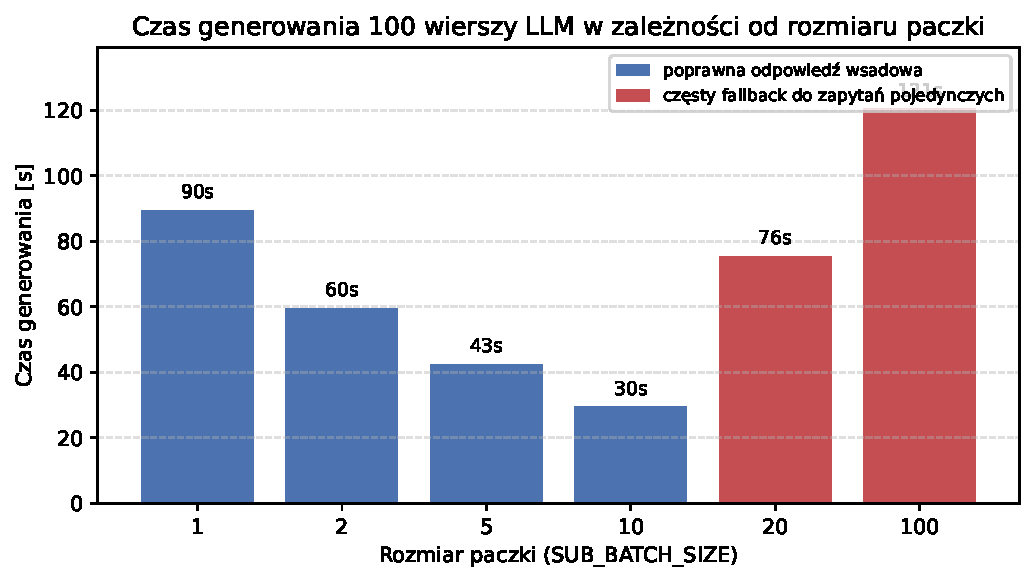
\includegraphics[width=0.85\textwidth]{images/batch_size_chart.pdf}
    \caption{Czas generowania 100 wierszy LLM w zależności od rozmiaru paczki}
    \label{fig:batch_size_chart}
\end{figure}

Wyniki zestawione w Tabeli \ref{tab:batch_size_comparison} i na Rysunku \ref{fig:batch_size_chart} pokazują wyraźną zależność: im więcej wierszy mieści się w jednym zapytaniu, tym krótszy jest łączny czas --- ale tylko do pewnej granicy. Przejście z paczki 1 na 10 skróciło generowanie z 90 s do 30 s, czyli około 3-krotnie. Każde kolejne zapytanie API niesie ze sobą narzut sieciowy i czas oczekiwania na odpowiedź modelu; grupowanie wierszy redukuje liczbę takich wywołań i dlatego daje realne przyspieszenie.

Od paczki 20 w górę trend się odwraca. Przy zbyt dużej liczbie wierszy w jednym prompcie model zaczął zwracać tablice \gls{JSON} o niepoprawnej długości -- zamiast dokładnie $N$ elementów otrzymywano krótsze lub dłuższe odpowiedzi. Silnik wykrywa ten błąd (porównanie \texttt{len(parsed\_array)} z oczekiwaną liczbą wierszy w paczce) i uruchamia mechanizm \textit{fallback}: uszkodzona paczka jest przerabiana ponownie, tym razem po jednym wierszu na zapytanie. Przy paczce 20 i 100 fallback uruchamiał się tak często, że łączny czas wzrósł do 76 s i 121 s --- wartości gorszych niż przy mniejszych, stabilnych paczkach.

Analiza wskazuje na dwa istotne wnioski. Po pierwsze, grupowanie wierszy w paczki skraca łączny czas generowania w porównaniu z wysyłaniem pojedynczych rekordów --- wariant sekwencyjny (\texttt{SUB\_BATCH\_SIZE=1}) okazał się najwolniejszy. Po drugie, zwiększanie rozmiaru paczki nie prowadzi monotonicznie do poprawy wydajności: przy zbyt dużych wartościach rośnie liczba błędów formatowania odpowiedzi, co wymusza kosztowny mechanizm \textit{fallback}. Dla testowanego modelu udostępnianego przez API OpenAI najkorzystniejszy czas uzyskano przy \texttt{SUB\_BATCH\_SIZE} równym 10; zakres 5--10 wierszy na zapytanie stanowi kompromis między liczbą wywołań API a stabilnością odpowiedzi. Wartość \texttt{SUB\_BATCH\_SIZE=15} zastosowana przy lokalnym serwerze Ollama (Tabela \ref{tab:llm_optimization_100}) została ustalona w odrębnych pomiarach --- potwierdza to, że optymalny rozmiar paczki zależy od dostawcy modelu i wymaga weryfikacji empirycznej w docelowym środowisku uruchomieniowym.

\subsection*{Porównanie wydajności Faker i LLM}
Kolejne pomiary wykonano na tym samym sprzęcie. Wykorzystano czterotabelowy schemat testowy \texttt{ecommerce\_llm\_\allowbreak schema}, w tym tabelę recenzji z polem \texttt{review\_text} generowanym przez \gls{LLM}.

\begin{table}[H]
    \centering
    \begin{tabular}{|l|c|c|c|}
        \hline
        \textbf{Typ danych}       & \textbf{Liczba wierszy} & \textbf{Czas (Faker)} & \textbf{Czas (\gls{LLM})}   \\
        \hline
        Proste (imię, adres)      & 1\,000                  & 0,8s                  & --                          \\
        \hline
        Proste                    & 10\,000                 & 5,2s                  & --                          \\
        \hline
        Złożone (z kontekstem AI) & 100                     & --                    & 52,24s (po optymalizacji)   \\
        \hline
        Złożone (z kontekstem AI) & 10\,000                 & --                    & 8\,038s ($\approx$2h 14min) \\
        \hline
    \end{tabular}
    \caption{Zestawienie czasów generowania danych strukturalnych i kontekstowych}
    \label{tab:performance_tests}
\end{table}

Jak widać w Tabeli \ref{tab:performance_tests}, generowanie danych przy użyciu algorytmów pseudolosowych (Faker) jest niezwykle szybkie i skalowalne liniowo. Wąskim gardłem systemu pozostaje generowanie treści przez \gls{LLM}, co potwierdza słuszność decyzji o zastosowaniu przetwarzania wsadowego z kontrolą współbieżności.

\subsection*{Alternatywny silnik --- vLLM}
Początkowe prace nad aplikacją oraz testy lokalne opierały się na serwerze Ollama \cite{ollama} --- narzędziu zaprojektowanym z myślą o prostocie obsługi i łatwym uruchamianiu modeli LLM na komputerach osobistych. Ollama wyróżnia się intuicyjnym interfejsem i prostym procesem instalacji, co doskonale sprawdza się przy deweloperskich eksperymentach. Jednakże w zastosowaniach chmurowych, wymagających dużej przepustowości i serwowania wielu równoczesnych zapytań, jego architektura nie oferuje optymalnej wydajności.

W celu maksymalizacji prędkości generowania w środowisku chmurowym przeprowadzono testy z wykorzystaniem vLLM \cite{vllm} --- biblioteki serwującej modele LLM, opracowanej na Uniwersytecie Kalifornijskim w Berkeley. vLLM różni się od Ollama podejściem architektonicznym: zamiast interfejsu zorientowanego na użytkownika końcowego, oferuje zaawansowany silnik zoptymalizowany pod kątem produkcyjnej wydajności i maksymalnego wykorzystania sprzętu.

Kluczowym mechanizmem vLLM jest \textit{PagedAttention} --- algorytm zarządzania pamięcią GPU inspirowany mechanizmami stronicowania pamięci z systemów operacyjnych. Standardowe podejście do obsługi mechanizmu uwagi \cite{attention_ml} w modelach LLM wymaga alokacji ciągłego bloku pamięci dla każdego zapytania, co prowadzi do fragmentacji i marnotrawstwa zasobów GPU. PagedAttention dzieli pamięć kontekstu KV-cache na małe, nieciągłe bloki, które mogą być dynamicznie przydzielane i zwalniane. Drugą istotną zaletą jest mechanizm \textit{continuous batching}, który dynamicznie łączy napływające zapytania w czasie rzeczywistym, bez konieczności czekania na skompletowanie całej paczki.

\subsubsection*{Konfiguracja vLLM na platformie Kaggle}
Wdrożenie vLLM w środowisku Kaggle wymagało rozwiązania dodatkowych problemów środowiskowych. Domyślna wersja vLLM (0.17) korzysta z biblioteki FlashInfer, która wymaga kompilacji kerneli CUDA w czasie wykonywania programu. System plików Kaggle, będący w dużej części środowiskiem tylko do odczytu, uniemożliwiał tę kompilację, powodując błędy budowania oprogramowania.

Rozwiązaniem okazało się zastosowanie starszej wersji vLLM (0.6.6), która zamiast FlashInfer wykorzystuje bibliotekę xFormers \cite{xformers}. xFormers dostarcza prekompilowane, wydajne implementacje operacji uwagi, co eliminuje konieczność kompilacji kerneli CUDA w czasie uruchamiania serwera.

Model Llama 3 8B-Instruct uruchomiono z podziałem tensorów na dwie karty Tesla T4 (\texttt{tensor-parallel-size=2}), co pozwoliło na wykorzystanie łącznie 32 GB pamięci VRAM. Aplikacja, dzięki oparciu komunikacji na standardzie OpenAI API, wymagała jedynie zmiany adresu URL serwera modelu oraz wyłączenia sztucznego podziału na paczki --- dotychczasowy interfejs i logika przetwarzania po stronie backendu pozostały niezmienione, delegując pełne zarządzanie ruchem do silnika vLLM.

\subsection*{Skalowalność dla dużych zbiorów danych}
W celu ostatecznego porównania wydajności wykonano próbę obciążeniową polegającą na wygenerowaniu bazy danych zawierającej 10\,000 wierszy przetworzonych przez \gls{LLM}. Testy przeprowadzono na dwóch platformach sprzętowych oraz z dwoma silnikami inferencji (Ollama i vLLM).

\begin{table}[H]
    \centering
    \begin{tabular}{|l|l|c|c|c|}
        \hline
        \textbf{Środowisko testowe} & \textbf{Silnik} & \textbf{Wierszy AI} & \textbf{Czas [s]} & \textbf{Czas/wiersz [s]} \\
        \hline
        Laptop (RTX 5060)           & Ollama          & 100                 & 52,24             & 0,52                     \\
        \hline
        Laptop (RTX 5060)           & Ollama          & 10\,000             & 8\,038,12         & 0,80                     \\
        \hline
        Kaggle (2x Tesla T4)        & Ollama          & 100                 & 178,02            & 1,78                     \\
        \hline
        Kaggle (2x Tesla T4)        & Ollama          & 10\,000             & 14\,860,23        & 1,49                     \\
        \hline
        Kaggle (2x Tesla T4)        & vLLM            & 100                 & 18,30             & 0,18                     \\
        \hline
        Kaggle (2x Tesla T4)        & vLLM            & 10\,000             & 1\,693,50         & 0,17                     \\
        \hline
    \end{tabular}
    \caption{Porównanie skalowalności w zależności od sprzętu i silnika}
    \label{tab:llm_scalability}
\end{table}

\begin{figure}[H]
    \centering
    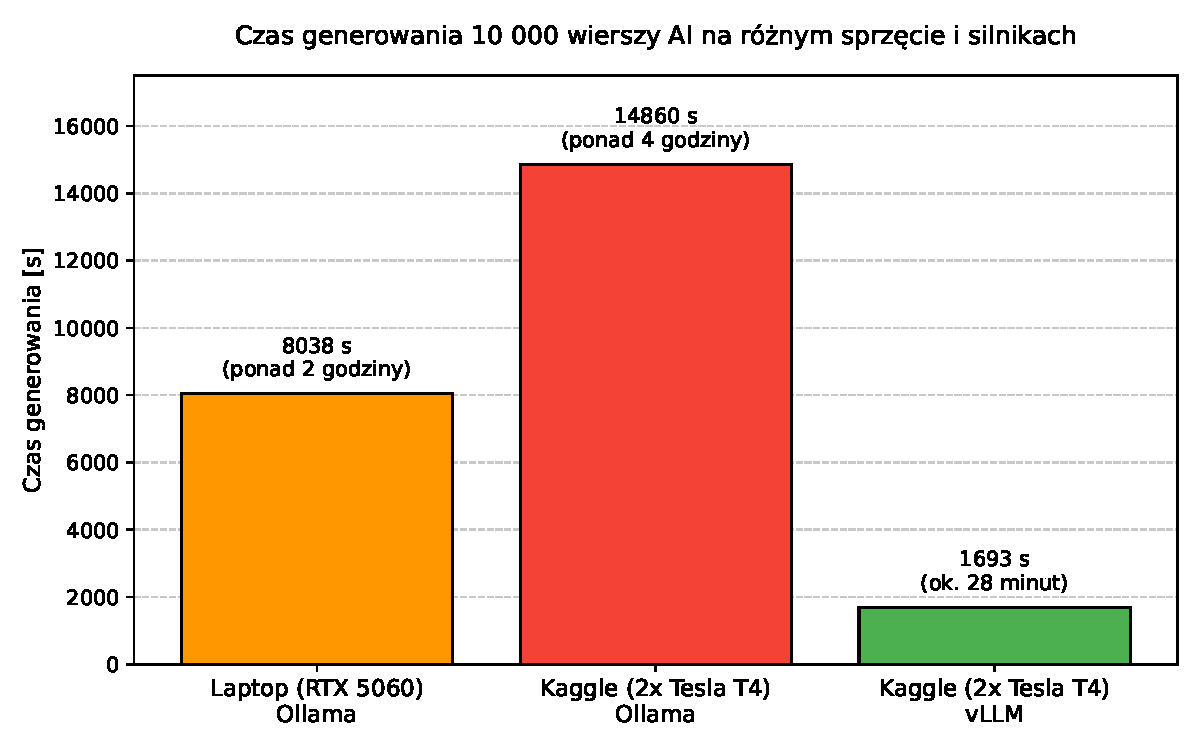
\includegraphics[width=0.85\textwidth]{images/hardware_comparison_chart.pdf}
    \caption{Wykres porównujący czas generowania 10\,000 wierszy AI na różnym sprzęcie}
    \label{fig:hardware_chart}
\end{figure}

Jak przedstawia Rysunek \ref{fig:hardware_chart}, wygenerowanie 10\,000 wierszy na laptopie z serwerem Ollama zajęło ponad 8\,038 sekund (nieco ponad 2 godziny). Długotrwałe obciążenie karty graficznej wiązało się ze zjawiskiem tzw. \textit{thermal throttling} (zabezpieczenie przed przegrzaniem obniżające taktowanie procesora), przez co średni czas utworzenia jednego wiersza wzrósł z 0,52 do 0,80 sekundy. Mimo to aplikacja zniosła ten test poprawnie i zapisała całą tabelę w pliku bazy SQLite.

Dla porównania, ten sam schemat z serwerem Ollama uruchomiono w darmowym środowisku chmurowym Kaggle, dysponującym dwoma kartami Tesla T4 (łącznie 32 GB pamięci VRAM). Pełna próba 10\,000 wierszy na Kaggle zajęła aż 14\,860 sekund (ponad 4 godziny). Różnica wydajności względem laptopa wynika ze specyfikacji sprzętowych --- karty Tesla T4 oparte są na architekturze Turing \cite{turing_microarchitecture} z 2018 roku, która nie posiada ulepszonych jednostek obliczeniowych obecnych w nowoczesnych kartach z serii RTX (architektura Ada Lovelace \cite{ada_lovelace_microarchitecture}).

Zastąpienie serwera Ollama przez vLLM na tej samej platformie Kaggle przyniosło drastyczną poprawę wydajności. Generowanie 100 wierszy AI skróciło się ze 178 do zaledwie 18,3 sekundy (przyspieszenie blisko 10-krotne), a pełna próba 10\,000 wierszy ze 14\,860 do 1\,693 sekund (około 28 minut zamiast ponad 4 godzin) --- przyspieszenie blisko 9-krotne. Średni czas na wiersz z vLLM (0,17 s) okazał się ponad 4-krotnie lepszy niż najlepsza lokalna konfiguracja Ollama na laptopie RTX 5060 (0,52 s). Wynik ten potwierdza, że mechanizmy PagedAttention i \textit{continuous batching} zaimplementowane w vLLM pozwalają na znacznie efektywniejsze wykorzystanie chmurowych zasobów GPU niż tradycyjne podejście serwera Ollama.


\section{Podsumowanie i wnioski}
\label{sec:summary}
Celem niniejszej pracy magisterskiej było zaprojektowanie i zaimplementowanie nowoczesnego narzędzia do generowania syntetycznych danych relacyjnych, wspieranego przez modele sztucznej inteligencji. Cel ten został osiągnięty poprzez stworzenie kompletnej aplikacji webowej, która integruje szybkość tradycyjnych generatorów z kreatywnością modeli \gls{LLM}.

\subsection{Osiągnięcia}
W ramach prac zrealizowano wszystkie założone wymagania funkcjonalne i niefunkcjonalne:
\begin{itemize}
    \item Hybrydowy silnik generujący: Stworzono elastyczny mechanizm łączący bibliotekę Faker, szablony Jinja2 oraz modele \gls{LLM} (OpenAI/Ollama). Pozwala to na generowanie danych o dowolnym stopniu skomplikowania --- od prostych typów liczbowych po złożone opisy tekstowe.
    \item Obsługa relacji: Zaimplementowano algorytm automatycznego rozwiązywania zależności między tabelami, co gwarantuje spójność referencyjną generowanych zbiorów danych.
    \item Wydajność: Dzięki zastosowaniu architektury asynchronicznej (Celery + Redis) oraz optymalizacji wsadowego generowania przez \gls{LLM}, system jest w stanie obsłużyć generowanie dużych zbiorów danych bez blokowania interfejsu użytkownika.
    \item Eksport i integracja z bazami danych: Zaimplementowano bezpośredni zrzut danych do PostgreSQL, MySQL, MSSQL oraz Oracle, a także eksport do plików \gls{JSON} i \gls{CSV}.
    \item Konteneryzacja: Całość rozwiązania została zamknięta w kontenerach Docker, co drastycznie upraszcza proces wdrożenia i konfiguracji w dowolnym środowisku.
\end{itemize}

Kod źródłowy aplikacji udostępniono w repozytorium GitHub (Załącznik~\ref{app:github}).

\subsection{Dalszy rozwój aplikacji}
Zrealizowany projekt stanowi solidną podstawę do dalszego rozwoju. Zidentyfikowano kilka obszarów, w których system mógłby zostać rozbudowany:
\begin{enumerate}
    \item Wsparcie dla baz NoSQL: Rozszerzenie mechanizmu eksportu o silniki dokumentowe (np. MongoDB) zwiększyłoby uniwersalność narzędzia w scenariuszach pozarelacyjnych.
    \item Generowanie na podstawie istniejącej bazy: Ciekawą funkcjonalnością byłaby inżynieria wsteczna --- podłączenie się do istniejącej bazy danych, automatyczne odczytanie jej schematu i wygenerowanie danych testowych ,,podobnych'' do danych produkcyjnych (z zachowaniem anonimizacji).
    \item Inteligentne wykrywanie typów: Wykorzystanie \gls{LLM} do automatycznej sugestii typów danych na podstawie samej nazwy kolumny (np. wpisując nazwę ,,pesel'', system sam proponuje odpowiedni generator regex).
\end{enumerate}

Podsumowując, stworzone narzędzie wypełnia lukę na rynku generatorów danych testowych, oferując unikalną możliwość generowania treści semantycznie poprawnych i kontekstowych, co jest kluczowe w dobie nowoczesnych aplikacji opartych na danych.

